%% grundlagen.tex
%% $Id: grundlagen.tex 28 2007-01-18 16:31:32Z bless $
%%

\chapter{Background \& Related Work}
\label{ch:Background}

\section{Body Temperature}
\label{Background:BodyTemperature}
In medical practice, temperature is one of the most frequently measured physical quantities.
By measuring temperature, one gains information about the internal energy of an object.
From the biophysical point of view, temperature measurement determines the changes in physical quantities that occur in a thermodynamic system \cite{dolibogComparativeAnalysisHuman2022}.
Temperature can be expressed in different scales.
These include Celsius, Fahrenheit, Kelvin, and Rankine \cite{grodzinskyUnderstandingFeverBody2020}.
The human body temperature range is usually between $36.5-37.5^\circ C$ ($97.7-99.5^\circ F$) \cite{hutchisonHypothermiaTherapyTraumatic2008}.
However, body temperature varies constantly and is dependent on many influencing factors such as gender, age, time of day, and many others \cite{sund-levanderNormalOralRectal2002}.
Likewise, the state of consciousness and emotions are decisive factor that significantly influences the body temperature \cite{barbosaescobarTemperatureEmotions2021}.
In addition, the position at which the body temperature is measured is crucial \cite{Physiologie9783137960072ZVAB}.
In order to keep the body temperature within the normal temperature range through internal and external factors, the body uses thermoregulation, through which the temperature is constantly adjusted by signals from the central nervous system.

\subsection{Thermal Regulation}
\label{Background:BodyTemperature:ThermalRegulation}
A vital body function is the possibility of regulation from the exchange of body heat \cite{grodzinskyUnderstandingFeverBody2020}.
Regulation occurs through a neural feedback system. 
In many parts of the body, sensory means detect cold and heat and transmit them via the central nervous system to the hypothalamus.
This then responds to potential temperature adjustments by triggering physiological activity. 
This can be associated with a gain or loss of heat, which maintains body temperature.
Major players in regulating body temperature are the cardiovascular system, the sudomotor control system, and skeletal muscles. 
The goal is to maintain body temperature within the range of $25^\circ C$ ($95^\circ F$) to $41^\circ C$ ($105.8^\circ F$) \cite{pierauTemperatursensibilitaet2001}. 
An excessive rise in body temperature (hyperthermia or hyperpyrexia), in which temperature regulation is no longer functioning, must be treated as a medical emergency.
The same applies if the body temperature drops below $35^\circ C$.

\subsection{Core Body Temperature}
\label{Background:BodyTemperature:CBT}
Core body temperature is the temperature of the body's internal organs, such as the heart, liver, and brain, and is a commonly used indicator of human health and endurance performance.
Unlike the body core temperature, the body surface temperature is more easily influenced by the ambient temperature and therefore cannot reflect the changes inside the body as well as the body core temperature.
Core body temperature can be measured invasively rectally, orally (oesophagus), in the pulmonary artery (with the use of a catheter), or in the urinary bladder \cite{moranCoreTemperatureMeasurement2002a}.
However, the gold standard is different.
The core body temperature of a healthy human body differs almost little from the temperature of the blood flowing in the pulmonary artery \cite{krizanacFemoroiliacalArteryPulmonary2013, holtzclawMonitoringBodyTemperature1993}.
This is exactly what is used as the gold standard for measuring body core temperature \cite{krizanacFemoroiliacalArteryPulmonary2013, holtzclawMonitoringBodyTemperature1993, fulbrookCoreBodyTemperature1997, maxtonEstimatingCoreTemperature2004}.
However, this comes with a few critical points.
Measuring the temperature of the blood flowing in the pulmonary artery involves an invasive and risky procedure that requires the insertion of an apulmonary artery catheter \cite{yeohRevisitingTympanicMembrane2017}.
This is strongly recommended in a medical hospital and nowhere else.
All of the previously mentioned methods are not comfortable for humans. 
In addition, it is difficult to make a measurement over a longer period of time with these in everyday life.

Body temperature can also be measured non-invasive.
The following methods are much more convenient, but the measurement accuracy suffers somewhat.
Measuring the body temperature non-invasive can be done on the axilla, the tympanic membrane, and the body surface \cite{moranCoreTemperatureMeasurement2002a}.
Usually, core body temperature is constant only in the body core and consequently cannot be determined outside only by temperature sensors \cite{niedermannPredictionHumanCore2014}.
Due to this, it is necessary to use several other values for the calculation of the core body temperature. 
These can include e.g. skin temperature and skin heat fluxes or the heart rate.
Niedermann achieved a root mean square deviation (rmsd) ranging from $0.28 ^\circ C$ to $0.34 ^\circ C$ for all environmental conditions in 2014 \cite{niedermannPredictionHumanCore2014}.
Therefore, a principal component analysis (PCA) was performed to extract uncorrelated variables that were subsequently used in a linear regression model. 
Six parameters, consisting of three skin temperatures, two skin heat currents, and heart rate, were selected as input variables to generate two principal components. 
The predictive power of these components for estimating core body temperature was evaluated using multiple regression analysis.

\subsection{Skin Temperature}
\label{Background:BodyTemperature:SkinTemperature}
When measuring body temperature, skin temperature is often used to measure body temperature.
This is the result of a dynamic equilibrium between the heat released during metabolic processes and transferred to the skin layer by thermal conduction and convection, the heat extracted from the environment, and the heat transferred to the environment by radiation, convection, and evaporation \cite{dolibogComparativeAnalysisHuman2022}.
The skin temperature can be measured by various sensors. 
These include the infrared sensors, but also the thermistors. 
Both are equal for purposes of clinical electrodiagnostic readings.
Thermistors offer better responsiveness and sensitivity in measurements.
Infrared thermistors, on the other hand, are more convenient in terms of speed and maneuverability \cite{burnhamThreeTypesSkinSurface2006}.
Because the skin is exposed to external influences, temperature differences can quickly occur.
This can be caused by cold or warm ambient air, but also by rain or other influences.
Measurements on the skin that cannot be easily influenced, such as the armpits, are suitable here.

\subsection{Temperature Measurements}
\label{Background:BodyTemperature:TemperatureMeasurements}
% TODO: General Temperature measurements of the human body
In General, the temperature of a human body will be measured with a thermometer.
There are multiple techniques available on which the temperature value will be calculated. 
These are divided into contact and non-contact thermometers.
For a detailed overview, take a look at chapter \ref{Background:TemperatureSensors}.
Body temperature is often measured in the armpit, mouth, rectum, ear, or forehead.
The temperature in the armpit is typically $36.6^\circ C$, in the mouth $36.9^\circ C$, and $37.1^\circ C$ in the ear \cite{dolibogComparativeAnalysisHuman2022}.
The rectal temperature testing method is the most accurate of all measurements, while non-contact forehead thermometers are considered the least accurate, and measurements are taken with them should be confirmed by other methods.
The minimum value of the standard error for the above methods is $0.1^\circ C$ [9].
Ear readings are assumed to be of similar accuracy when compared to the rectal method, which is most commonly used in infants, the correct value is usually $37.1^\circ C$ \cite{dolibogComparativeAnalysisHuman2022}.

% Ear based temperature measeurements
Ear-based temperature measurement uses a sensor to measure the temperature of the ear canal. 
The approach has a number of advantages over other measurement positions.
First, it is a non-invasive measurement procedure, which allows measurement nearly inside the body with the least amount of hematoma.
Second, the measurement is much more promising compared to other non-invasive alternatives, where many factors can contribute to falsifying the final result \cite{ganioValidityReliabilityDevices2009, craigTemperatureMeasuredAxilla2000}. 
However, it is essential to note that the accuracy of temperature measurement may depend on factors such as the positioning of the thermometer and the presence of earwax or other obstructions in the ear canal.

% \subsubsection{Temperature Measurements on the Tympanic Membrane}
The tympanic membrane is a thin membrane that separates the middle ear from the external auditory canal. 
The artery called the external carotid artery runs near the external auditory canal and radiates heat, which is why measuring the temperature at the tympanic membrane has a promising chance of determining body temperature \cite{yeohRevisitingTympanicMembrane2017}.

Since measuring body temperature at the tympanic membrane is a non-invasive measurement method, it is already being investigated as a possible replacement for currently accepted methods.
This could be a safe and very convenient way of measuring core body temperature, but to date it is not de-facto due to unresolved problems.
These include the accuracy and stability compared to measurements at other locations \cite{maxtonEstimatingCoreTemperature2004, fulbrookCoreBodyTemperature1997, mumaComparisonRectalAxillary1991, rothAgreementRectalTympanic1996}.
Benzinger \cite{benzingerHeatRegulationHomeostasis1969, benzingerClinicalTemperatureNew1969, benzingerPhysicalHeatRegulation1959} first demonstrated the feasibility of tympanic membrane measurement as an indicator of core body temperature using a thermocouple temperature probe that engages the surface of the tympanic membrane with the ear canal sealed from the environment.
For this, Benzinger made measurements of tympanic membrane temperature obtained from his probe and measurement approach and showed them to be stable, reproducible, and responsive to thermal stresses of various types.
However, there are other studies at a later date that refute individual assumptions of this study.
McCaffrey et al. \cite{mccaffreyEffectHeadSkin1975} and Nielsen \cite{nielsenNaturalCoolingBrain1988} showed that head cooling reduces the body core temperature when measured with exactly the procedure of Benzinger.
McCaffrey et al. however, also showed that by heating and cooling localized regions of the head, infrared measurement of temperature at the tympanic membrane of human subjects was not proportionally affected by changes in head skin temperature.
This suggests a contradiction, which means that this method may not be a good predictor of core body temperature because it depends on other, as yet unknown, variables.
Brinnel and Cabanac \cite{brinnelTympanicTemperatureCore1989} and Sato et al. \cite{satoReexaminationTympanicMembrane1996}, however, provided data showing that measurements for this purpose are still reliable if the measurement point on the tympanic membrane is carefully chosen. 
Brinnel and Cabanac proposed that the lower anterior quarter of the tympanic membrane (Figure \ref{fig:tympanic_membrane_mp}) has a higher temperature on the surface of the tympanic membrane and temperature measurement from a point in this area is the least sensitive to head cooling.
\begin{figure}[t]
    \centering
    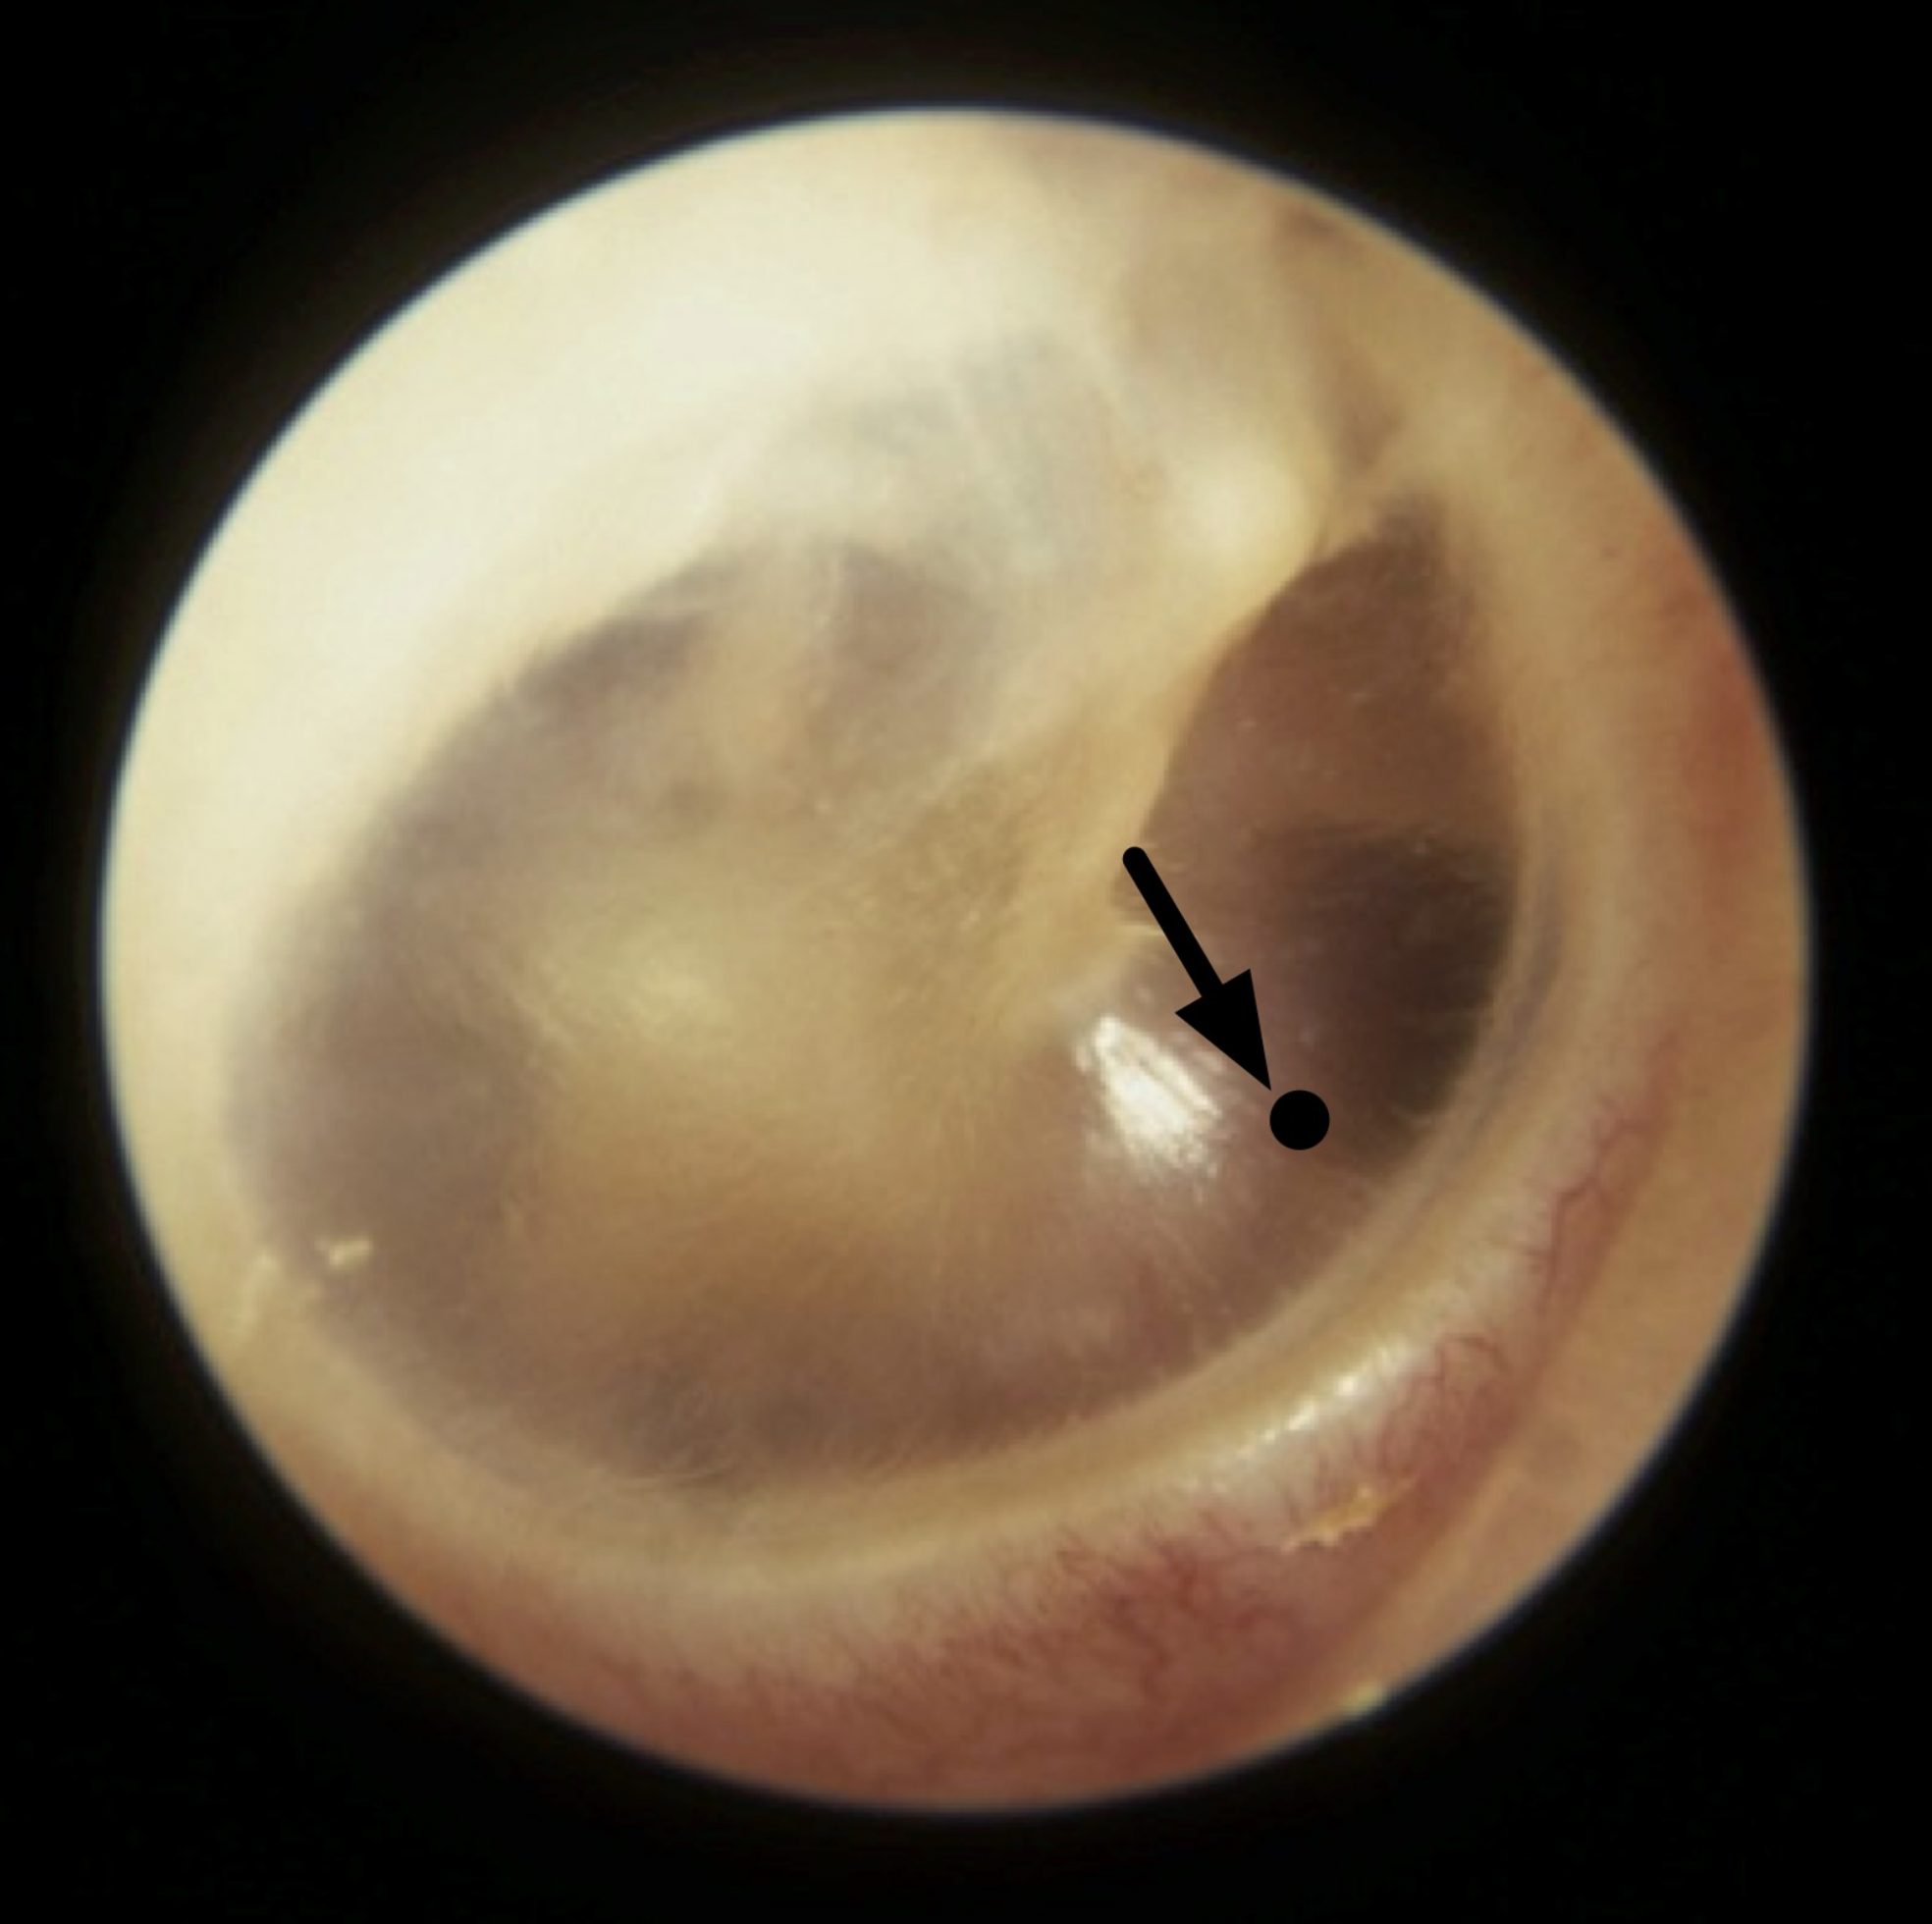
\includegraphics[scale=0.15]{thesis-doc/images/tympanic_membrane_mp.png}
    \caption{Caption}
    \label{fig:tympanic_membrane_mp}
\end{figure}

% das paper is von 1991, vllt schon zu alt und unrelevant
% TODO: \cite{ComparisonPulmonaryArtery}

% hier bei der comparison gehts um mittelohrentzündungen
% TODO: \cite{kimComparisonBilateralEardrum2022}

% das paper is von 1999, vllt schon zu alt und unrelevant
% TODO: \cite{childsTympanicMembraneTemperature1999}

Temperature sensors are used to measure the temperature of a particular object or environment.
They are widely used in many applications, such as industrial, medical, or scientific contexts.
Temperature sensors detect changes in temperature and convert this into a measurable signal.
There are various types of temperature sensors, including contact and non-contact sensors.

Contact sensors measure temperature by maintaining physical contact with an object and measuring the temperature there.
Contact sensors can be divided into 3 types: Thermocouples, Thermistors, and Resistance Temperature Detectors (RTDs). 
Thermocouples measure the voltage generated by two different metals when they are exposed to different temperatures.
RTDs measure changes in the electrical resistance of a metal wire when it has temperature changes.
Thermistors are semiconductor devices whose electrical resistance changes with temperature.

Non-contact sensors, on the other hand, do not require contact with the object being measured. They are also known as infrared sensors.
Non-contact sensors measure the emitted infrared radiation from an object and convert it into a measurable signal.
Most often, the sensors are used when contact with an object is not desirable or practical, such as can often be useful in a medical or scientific research context. 
This is also the case in this work, as contact with the tympanic membrane, for example, is not desired.
Non-contact sensors can be roughly divided into two categories: IR sensors and optical pyrometers.
IR sensors are devices that detect and measure the amount of infrared radiation emitted by an object. They operate on the principle that all objects emit infrared radiation in proportion to their temperature. 
Optical pyrometers, on the other hand, measure temperature by detecting the color of light emitted by an object. They work on the principle that the color of light emitted from a hot object changes as the temperature of the object changes.
However, the current classification here is very crude.
In addition to those mentioned above, there are, for example, fiber optic sensors and acoustic sensors.

When choosing the right sensor for a particular application, some things have to be considered.
Accuracy, response time, and range are important variables.
Depending on the requirement profile, the right sensor can be selected based on the parameters.
In the following, the optical temperature sensors, as well as the RTDs are described in more detail, since they are very important in this work.

\subsection{Optical Temperature Sensors}
\label{Background:TemperatureSensors:OpticalTS}
Optical temperature sensors, also known as optical pyrometers, measure temperature by detecting the color of light emitted from an object. 
This is based on the assumption that the color of the emitted light is different depending on the temperature.
Typically, this is done using a lens that focuses the emitted light from the object onto a detector, which then analyzes the color of the light. 
This is then ultimately used to determine the temperature.
This type of sensor is typically used in applications where contact with the object being measured is difficult or impossible, such as in space, harsh environments, or just where contact is not wanted.
Thus, non-contact measurements are possible, which is essential when measuring the temperature of the tympanic membrane.
Another advantage of optical temperature sensors is that moving objects can still be measured as long as the sensor continues to point at the object.
However, this requires a line of sight to the measured object.
In addition, accuracy can be affected by reflective surfaces or atmospheric conditions, which should not be a problem if the measurement is primarily in the ear.

\subsubsection{MLX}
\label{Background:TemperatureSensors:OpticalTS:MLX}
The MLX90632 sensor is an infrared thermopile temperature sensor.
It measures temperature without requiring contact with the skin. 
This is done by means of an infrared sensor. 
The sensor is based on a microelectromechanical system (MEMS), which is used to detect thermal radiation in the infrared spectrum emitted by the object to be measured \cite{melexisMLX90632FIRSensor2021}.
The MLX90632 has a small form factor and low power consumption, which is well-suited for small devices.
In addition, the sensor has a very high accuracy of $\pm 0.5 ^\circ C$ from $-20 ^\circ C$  to $100 ^\circ C$.
Here the sensor can resolve in $0.02 ^\circ C$ steps.
Another immense advantage is the simultaneous measurement of 2 temperature values at the same time.
This is possible because 2 sensor elements are directly installed in the MLX90632.
This enables the measurement of one object, such as the skin temperature, and the ambient temperature.
However, it is also possible to measure 2 different body parts at the same time.
In order to be able to integrate the sensor optimally into a system, an I2C interface is available so that a microcontroller can communicate easily.
Overall, the MLX90632 sensor provides a versatile and accurate solution for non-contact temperature measurement in a variety of applications, including medical, industrial, and consumer electronics.

\subsection{Thermal Resistance Temperature Detectors}
\label{Background:TemperatureSensors:ResistanceTD}
Thermal resistance temperature detectors operate by measuring changes in electrical resistance as a function of temperature. 
This type of sensor is typically used in applications where high accuracy is required, such as laboratory environments or medical equipment.
They provide high accuracy and cover a wide range of temperature measurements.
However, contact measurement is required here, which limits temperature measurement to stationary objects.
Furthermore, thermal resistance temperature sensors have a slow response time, which makes real-time measurement somewhat difficult.

In summary, optical temperature sensors are useful in situations where contact with the object being measured is difficult or impossible, while thermal resistance sensors are suitable for applications that require high accuracy and a wide temperature measurement range. 
Ultimately, the choice between these two types of sensors depends on the specific requirements of the application.

Here in the master's thesis, optical temperature sensors are suitable because they do not require direct contact points, which is essential when measuring temperature on the tympanic membrane.

\section{Sensing with Earables}
\label{Background:SensingWithEarables}
Earables belong to the class of wearables and are a type of wearable device that is worn in or around the ears. 
They typically have a number of sensors that allow them to collect data about the wearer's physiology and activity. 
The most common sensors in earables include accelerometers, gyroscopes, and heart rate monitors. 
These sensors can be used to track the wearer's movements, monitor their heart rate, and provide other types of health data.
Earables are portable, lightweight, and small, which allows them to be worn easily for long periods of the day \cite{roddigerSensingEarablesSystematic2022a}. Thus, data can be tracked over a longer period of time. In addition, earables have the advantage of being worn on the ear, which together with the head are automatically stabilized during movements and thus have less motion disturbances and artifacts \cite{grossmanFrequencyVelocityRotational1988, kavanaghRoleNeckTrunk2006a}.
The position on the ear brings a lot of potential. For one thing, the ear is very close to the brain and blood vessels, which allows accurate measurement of brain activity, cyclic blood flow, and related properties \cite{ferliniInEarPPGVital2022}.
In addition, it is possible to detect the perception of a variety of facial, neck, and eye muscle activations \cite{andoCanalSenseFaceRelatedMovement2017}, as well as the input of head movements \cite{andoCanalSenseFaceRelatedMovement2017}, facial gestures \cite{matthiesEarFieldSensingNovelInEar2017}, mouth movements \cite{sunTeethTapRecognizingDiscrete2021a}, and instantaneous \cite{bleichnerConcealedUnobtrusiveEarCentered2017, phamWAKEBehindtheearWearable2020Concealed, unobtrusive ear-centered EEG acquisition: cEEGrids for transparent EEG}. 
Because of the ease of accessibility with the hand \cite{kikuchiEarTouchTurningEar2017, xuEarBuddyEnablingOnFace2020}, interactions with the hand on the ear can be used to trigger actions \cite{lissermannEarPutAugmentingEarworn2014}.
In summary, earables are capable of triggering a variety of processes of the skeleton (e.g., gait \cite{atallahGaitAsymmetryDetection2014}), muscles (e.g., facial expressions \cite{matthiesEarFieldSensingNovelInEar2017}), nerves (e.g. Brain activity \cite{debenerUnobtrusiveAmbulatoryEEG2015}), endocrine system (e.g. , emotions \cite{athavipachWearableInEarEEG2019}), cardiovascular system (e.g. , blood pressure \cite{atallahValidationEarwornSensor2012}), respiratory system (e.g. , breathing \cite{roddigerRespirationRateMonitoring2020}), and digestive system (e.g. , food intake \cite{gaoIHearFoodEating2016}).

In 2022, Röddiger et al. noted the current state of research on sensing with earables \cite{roddigerSensingEarablesSystematic2022a}.
A systematic literature review of 271 peer-reviewed research articles was made receiving a better understanding of the current state of research on this topic.
The research area was divided there into four categories (Figure \ref{fig:sensing_with_earables_overview}), which will now be explained in more detail.

\begin{figure}[t]
    \centering
    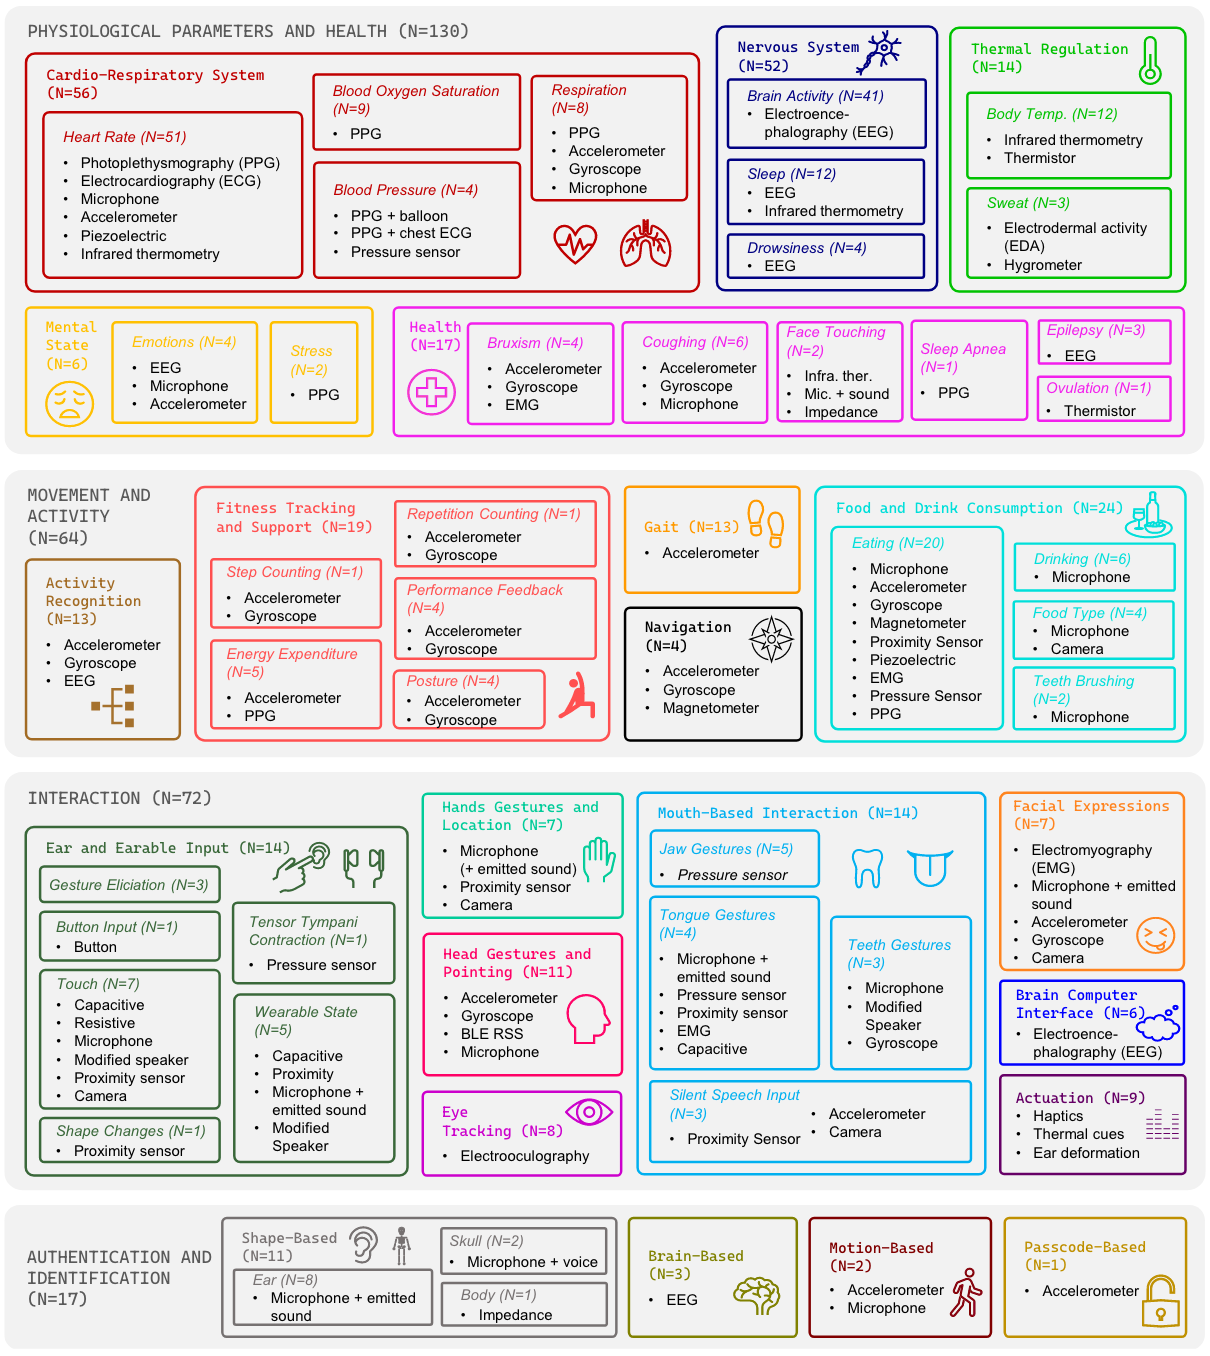
\includegraphics[scale=0.3525]{thesis-doc/images/sensing_with_earables_overview.png}
    \caption{Overview map of sensing with earables. The map displays all phenomena current research is about divided into the main four categories. For each phenomena, there is a number (N), which describes the available articles and all the used sensors used to detect these phenomena \cite{roddigerSensingEarablesSystematic2022a}.}
    \label{fig:sensing_with_earables_overview}
\end{figure}

\subsection{Physiological Monitoring and Health}
\label{Background:SensingWithEarables:Physiological}
The first categorical classification of sensing with earables is physiological parameters and health.
The use of ear-worn sensors to track and maintain personal health by monitoring various physiological parameters is considered.
The parameters are categorized according to human body functions such as the cardio-respiratory system, nervous system, thermoregulation, mental status, and health monitoring.
The cardio-respiratory system is divided into the areas of heart rate, blood oxygen saturation, respiration, and blood pressure.
All these areas can be classified, for example, with a PPG (photoplethysmography). 
When determining the heart rate, a microphone, an accelerometer, an infrared thermometer, the piezoelectric, or an EEG (electrocardiography) can be used.
The nervous system includes the classification of brain activity, sleep, or drowsiness. 
All are determined using an EEG. When classifying sleep, an infrared thermometer can also be used for classification. 
The most researched area here in the context of earables is brain activity.
The 3rd subcategory in the physiological parameters and health represents the mental state.
This has not yet been researched that far in the context of earables with 6 reference papers.
Emotions can be recognized using an EEG, a microphone, or an accelerometer, and even stress using a PPG.
Another subcategory is health which is divided into bruxism, coughing, face touching, sleep apnea, epilepsy, and ovulation.
Sensors such as an accelerometer, a gyroscope, a microphone, an EEG, PPG, or an infrared thermometer are used here.
For further details please refer to the original paper \cite{roddigerSensingEarablesSystematic2022a}.
The last part of the physiological parameters and health is thermal regulation. A distinction is made here between body temperature and perspiration. An EDA (electrodermal activity) and a hygrometer are used for sweating.
When classifying body temperature, an infrared thermometer, and a thermistor are used.
Due to the body temperature being the most crucial part of this thesis, this part will now be focused in more detail.

\paragraph{Body temperature}
\label{Background:SensingWithEarables:Physiological:BodyTemperature}
Bestbier and Fourie \cite{bestbierDevelopmentVitalSigns2018} applied the principle to a wearable form factor and achieved a small mean error of only $0.02$ $\pm$ $0.52 ^\circ C$. 
They used the TMP006 infrared sensor, which points directly at the eardrum. 
The thermophilic voltage and the temperature sensor were made digitally available via hardware registers, from which the object temperature can be calculated. 
This reflects the temperature of the tympanic membrane after calibration.
However, the accuracy varies greatly between individual positions, which is attributed to the orientation of the sensor due to a wide variety of auditory canals.
This problem was solved by implementing intraparticipant calibration.
This should allow the sensor to self-calibrate automatically and improves the standard error by $56\%$ (from $0.5125 ^\circ C$ to $0.29 ^\circ C$) and the correlation coefficient from $0.4667$ to $0.8684$.

However, user-defined calibration is needed because the shape of the ear canal is different for each individual \cite{bestbierDevelopmentVitalSigns2018, luekenPhotoplethysmographybasedInearSensor2017, matsumotoEarbudtypeWearableHearable2019}.
Luken et al. integrated TI's TMP007 into the proposed measurement system to obtain information about human core temperature variation at a rate of $33 Hz$ \cite{luekenPhotoplethysmographybasedInearSensor2017}.
For individual calibration purposes, the voltage difference of the thermopile element and the chip temperature was transmitted in addition to the recorded object temperature.
However, the temperature was not further calibrated or processed in this work \cite{luekenPhotoplethysmographybasedInearSensor2017}.
Alternatively, surface skin temperature at the mastoid can be determined with high accuracy ($0.03 ^\circ C$ mean error) \cite{atallahErgonomicWearableCore2018}.
% TODO: read atallahErgonomicWearableCore2018 paper and insert content
A known factor for changes in body temperature is considered in earable research to be the response to external weather conditions \cite{barralonAugmentedHearingAssistance2015, boanoNoninvasiveMeasurementCore2013, celikEvaluationBehindtheEarECG2016} and during physical activities \cite{boanoNoninvasiveMeasurementCore2013, chagllae.MeasurementCoreBody2018, celikEvaluationBehindtheEarECG2016, matsumotoEarbudtypeWearableHearable2019, sugimotoDevelopmentWirelessSensing2011}.
% TODO: read all the previous papers and explain a lot more here!
These findings enable a number of applications that perform some important functions, such as alerting or vital signs and parameter tracking based on the identified relationships.
In addition, the relationship between body temperature recorded at the ear and ovulation (see subsection 4.5.6) and sleep (see subsection 4.2.2) has been demonstrated.
% TODO: remove the above sentence and insert content from sections mentioned

\subsection{Movement and Activity}
\label{Background:SensingWithEarables:Movement}
% TODO: Go into more detail for each section here

\subsection{Interaction}
\label{Background:SensingWithEarables:Interaction}
% TODO: Go into more detail for each section here

\subsection{Authentication and Identification}
\label{Background:SensingWithEarables:Authentication}
% TODO: Go into more detail for each section here

\subsection{Sensing Platforms}
\label{Background:SensingWithEarables:SensingPlatforms}
% TODO: Hier abschnitt zu sensing platforms, wie z.B OpenEarable

% https://media.digikey.com/pdf/Data%20Sheets/Excelitas%20PDFs/TPiS_1S_1385.pdf

% address translator weiter hinten, wo ich die implementierung ändere
% \subsection{Address translator}
% da die sensoren alle die gleiche addresse haben werden brauche wir da noch so address übersetzter, ich denke sopwas in die richung: 
% https://www.analog.com/media/en/technical-documentation/data-sheets/4316fa.pdf